% !TeX spellcheck = de_DE
% !TeX TXS-program:compile = txs:///lualatex/[-shell-escape]


\documentclass[11pt]{scrartcl}

\usepackage[ngerman]{babel} % Use this if your write in German

\usepackage{minted}
\usepackage{abstract}
\usepackage[colorlinks]{hyperref} % Gives us \autoref and \href
\usepackage{graphicx} % Gives us \includegraphics

\title{Belegarbeit Laborprojekt - Grundlagen der Programmierung HTW}
\author{Lennard Wittenberg}

\begin{document}

\maketitle

\begin{abstract}
Belegarbeit zum Laborprojekt. Es enthält eine Beschreibung der Problematik, Vorgehen und Lösungswege bei der Implementation und ein Fazit.
\end{abstract}
%
\newpage
%
\tableofcontents
%
\newpage
%
\section{Einführung}
%
\label{sec:intro}
Im Rahmen des HTW Moduls CE22 "Grundlagen der Programmierung Projekt" wird in dieser Belegarbeit Mein Ansatz bei der Implementierung des mathematischen Algorithmus von John Conway dargestellt.
Zu Referenz ist unter diesem \href{https://gitlab.rz.htw-berlin.de/Lennard.Wittenberg/c-wise-lennard-wittenberg/-/blob/main/projects.pdf}{Link} das Aufgabenblatt zu finden.
%
\subsection{Aufbau der Arbeit}
1.) Im ersten Abschnitt wird das Game of Life vorgestellt. Was ist das Game of Life? Was sind die Regeln des Game of Life? Vorstellung einiger Besonderheiten\\
2.) Im zweiten Abschnitt werden meine Ziele und Ideen bei der Umsetzung vorgestellt.\\
3.) Im dritten Abschnitt wird mein Vorgehen bei der Lösung der Problematik detailliert beschrieben.\\
4.) Im letzten Abschnitt gibt es einen Rückblick auf das Projekt und ein Fazit.
%
\section{Was ist das Game of Life}
\label{sec:info}
Das Game of Life (Lebensspiel) ist eine Computersimulation. Lebewesen bzw. Zellen verteilen sich auf einem unbegrenzten, karierten Feld. Je nach Nachbarschaft bleiben sie am Leben, sterben oder bringen neues Leben hervor.
Game of Life kann auch als zellulärer Automat angesehen werden, bei dem der Zustand einer Zelle vom eigenen Zustand und von dem der Nachbarzellen abhängt. 
Das Spiel wurde 1970 vom englischen Mathematikprofessor John Conway entwickelt.
\begin{figure}
\centering
\label{fig:Abb1}
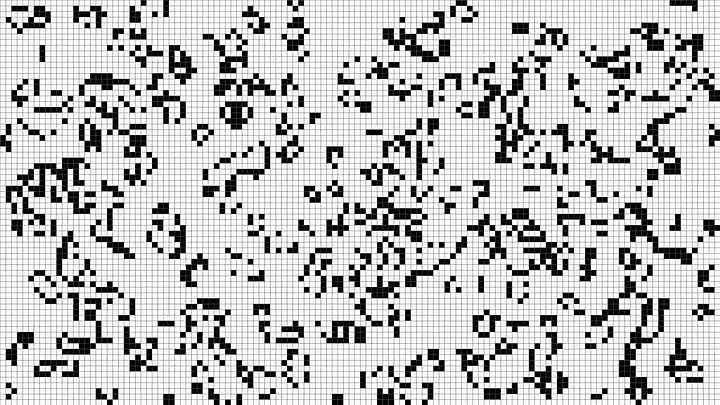
\includegraphics[width=0.45\textwidth]{0 i4NRQkJRLh-21WNN.png}
\end{figure}
\subsection{Regeln}
Jede neue Generation wird nach einer Überlebensregel (I), einer Sterberegel (II) und einer Geburtsregel (III) ermittelt.
Die Zellen befinden sich dabei auf einem "Koordinaten\-Netzt". haben bis zu 8 Nachbarn. Je nachdem, ob sich eine Zelle am Rand oder in der Ecke des Netzes, kann die Anzahl der Nachbarn variieren. 
1. Fall: Eine Zelle ist lebendig.\\ 
(I) Das Lebewesen in dieser Zelle überlebt, wenn es 2 oder 3 Nachbarn hat.\\ 
(II) Das Lebewesen stirbt, wenn es 0, 1, 4, 5, 6, 7 oder 8 Nachbarn hat. \\
(Bei keinem oder einem Nachbarn stirbt es aus Einsamkeit, bei 4 bis 8 wegen Überbevölkerung.)\\
2.Fall: Eine Zelle ist tot.\\ 
(III) Gibt es zu dieser Zelle genau 3 Lebewesen in den Nachbarzellen, so entsteht hier eine neue Zelle. In allen anderen Konstellationen bleibt sie tot.\\
\begin{figure}
\centering
\label{fig:Abb2}
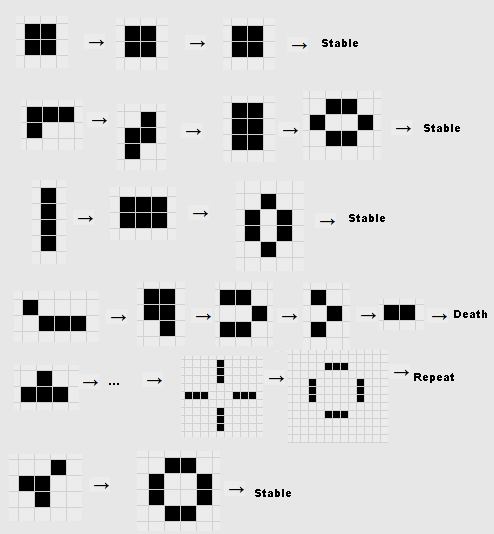
\includegraphics[width=0.45\textwidth]{4life2.png}
\end{figure}
Ein Beispiel für die Entwicklung von Generationen ist \ref{fig:Abb2} in diesem Bild zusehen.
\subsection{Kategorien}
Im Game of Life gibt es verschiedene Kategorien von Figuren beziehungsweise Muster, die entweder zufällig nach mehreren Generationen entstehen oder initial erschaffen wurden. Einige der wichtigsten beziehungsweise häufigsten möchte ich hier einmal vorstellen.
Stilllifes:\\
Die stabilen Populationen enthalten nur Lebewesen mit 2 oder 3 Nachbarn und ändern sich nicht mehr. Sie hei\ss en nach Conway Stillleben.\\
Oszillatoren:\\
Ein Oszillator ist ein Muster, das nach einer endlichen Anzahl von Generationen in seinen ursprünglichen Zustand mit derselben Ausrichtung und Position zurückkehrt. Somit wiederholt sich die Entwicklung eines solchen Musters auf unbestimmte Zeit periodisch.\\
Space ships:\\
Ein endliches Muster wird als Raumschiff bezeichnet, wenn es nach einer bestimmten Anzahl von Generationen in derselben Ausrichtung, aber an einer anderen Position wieder auftaucht. Die kleinste dieser Generationen wird als Raumschiffsperiode bezeichnet.\\
Bei Interresse findet man unter diesem \href{https://en.wikipedia.org/wiki/Conway\%27s_Game_of_Life#Examples_of_patterns}{Link} eine genauere und umfangreichere Auflistung von Mustern.
%
\section{Ziele und Ideen}
Da ich allein gearbeitet hatte und begrenzte Zeit hatte, habe ich mich dafür entschieden, auf eine Umsetzung mit SDL2 zu verzichten und stattdessen Print to Terminal zu verwenden. Darüber hinaus war mein Ziel, nicht nur die Regeln des Spiels fehlerfrei zu gewährleisten, sondern auch Fehler so effizient wie möglich abzufangen und zu verarbeiten. Aufgrund meiner Entscheidung, auf SDL2 zu verzichten, musste ich einen Weg finden, die Verwendung des Programms Nutzern zuvorkommend zu gestalten. Als Nebenziel wollte ich meinen Code nach dem DRY-Code System und mit einer hohen Wiederverwendbarkeit gestalten.
\section{Vorgehen und Lösungswege}
Die Beschreibung meines Vorgehens ist in Phasen eingeteilt und jede Phase bekommt einen eigenen Unterabschnitt.
\subsection{Phase 1 - Konzept und Plannung}
Zu Beginn meiner Arbeit habe ich das Internet nach Tutorial-Videos und Artikeln durchsucht, um einen besseren Eindruck vom Projekt zu erlangen und die Grundkonzepte des Game of Life zu verstehen. Zu anderen habe ich nach einer Grundstruktur gesucht, welche ich ebenfalls für mein Projekt nutzen könnte.
Danach hatte ich drei Ergebnisse, mit denen ich weiterarbeiten wollte.
Die Seite \href{http://www.mathematische-basteleien.de/gameoflife.htm}{Mathematische Basteleien} ist ideal, um sich einen Überblick über das Game of Life zu verschaffen und die Grundlagen zu verstehen.
Auf dem \href{https://www.geeksforgeeks.org/program-for-conways-game-of-life/}{Geeks for Geeks} Portal habe ich ein gutes kleines Beispiel für die Implementation des Game of Life gefunden. Ich habe den Code
dieser Seite als Grundkonzept verwendet und im Laufe meiner Arbeit immer wieder Teile des Code bei meiner Implementation verbaut.
Die Guithub Instanz von \href{https://github.com/noahhaasis/conwaysGameOfLife}{noahhaasis} hat mir dabei geholfen mir einen Eindruck zu verschaffen, wie vollständiges Game of Life aussehen könnte. Auch hier habe keinere Teile in meine Arbeit eingebaut allerdings in diesem Fall nur in sehr kleinen Ausschnitten.
\subsection{Phase 2 - Anfang}
Initial habe ich mit vier Dateien gearbeitet. Eine Main-Datei eine Datei, die alle Hauptfunktionen des Projekts beinhaltet, die dazu gehörige Companion-Datei und eine Datei, die sämtliche Unit-tests beinhaltet.
Ich diesem Abschnitt liegt der Fokus auf der Companion-Datei gol\_board.h\\
In dieser Datei sind alle wichtigen Hauptfunktionen definiert, die für die Arbeit mit dem Game of Life vonnöten sind. Darüber hinaus wird hier auch die Struktur, die das Spielfeld darstellen soll, definiert. Die Struktur hat zwei zweidimensionale integer Pointerarrays und int Variablen als Mitglieder. Die Arrays repräsentieren das Spielnetz.  Das erste Array stellt die aktuelle Generation dar und das zweite Array stellt die darauffolgende Generation dar. Die int Variablen speichern die maximalen Werte der Netzdimensionen. Dazu ist wichtig zu wissen, dass das Netz wie ein Koordinatensystem in Quadratform funktioniert. Wobei der Nullpunkt die obere linke Ecke darstellt und die untere rechte Ecke die Grenzen des Netzes.
Die drei Hauptfunktionen haben die folgenden Aufgaben:\\
1. Das Spielfeld initialisieren und alle Zellen im Netz zu Beginn als Tot deklarieren. Zudem werden die maximalen Dimensionswerte bestimmt.\\
2. Alle lebenden Zellennachbarn einer Zelle bestimmen.\\
3. Die Spielregeln im Bezug auf alle Zellen umsetzten und bestimmen, welche Zellen sich wie verhalten sollen.\\
Die genaue Umsetzung und alle Hilfsfunktion werden in den folgenden Abschnitten erläutert. Die finale \href{https://gitlab.rz.htw-berlin.de/Lennard.Wittenberg/c-project-wise-lennard-wittenberg/-/blob/main/gol_board.h}{Datei}  
\subsection{Phase 3 - Umsetzung}
Grundsätzlich verlief meine Arbeit nach dem folgenden Prinzip. Baustein oder Idee konzeptionieren, diese dann umsetzen und dann, wenn der Code kompiliert, diesen dann testen. Wobei der der zweite und dritte Schritt immer wieder wiederholt wird, bis das Konzept umgesetzt wurde.
Dazu habe ich die Main-Datei zum i/o Debugging genutzt. Im diesem Abschnitt werden die einzelnen Funktionen und deren Umsetzung konkret beschrieben.
\subsubsection{initialize\_board und delete\_board}
Aufgabe: Das Spielfeld initialisieren und alle Zellen im Netz zu Beginn als Tot deklarieren. Zudem werden die maximalen Dimensionswerte bestimmt.
Zu dieser Funktion wird ebenfalls ein Gegenstück benötigt, welche den belegten Speicher der Pointer wieder freigibt.\\
toten Zellen wird der Werte 0 zugewiesen und lebenden Zellen wird eine 1 zugewiesen.\\
Code:\\
Die initialize\_board Funktion nimmt drei Variablen und gibt eine Instanz der Spiel Struktur zurück. Die erste Variable ist eine Struktur des Spielfeldes. Die zweite und dritte Variable sind Integer Variablen, 
die die Grenzen des Spiel Netzes darstellen. Auf diese Werte haben Nutzer keinen Einfluss. Innerhalb der Funktion wird eine zweidimensionale integer Matrix mit zwei for-loops, mit den übergebenen int Parametern, erzeugt.
Der besetzte Speicher wird dann den Struktur Mitgliedern zugewiesen. Hier bin ich zu ersten Mal auf einen gro\ss en Fehler gesto\ss en. Während meiner Unit-tests habe ich durchgehend den Fehler erhalten, dass ein zugewiesener Speicherplatz nicht zweimal gelöscht werden. Dadurch ist mir aufgefallen, dass es zu Komplikationen kommt, wenn ich den Pointer Mitgliedern den selben Speicherplatz zuweise. 
Abschlie\ss end werden die übergebenen int Parameter den Struktur Mitgliedern zugewiesen, diese sind in späteren Funktionen wichtig und die bearbeitete Spielstruktur wird zurückgegeben.\\
delete\_board ist sehr simple. Über ein for-loop werden die einzelnen Dimensionen der Pointerarrays freigegeben und abschlie\ss end werden die Pointer als solche freigegeben. Die Funktion hat keinen Rückgabewert und nimmt eine Spielnetzstruktur als Parameter, welche gelöscht werden soll.      
\subsection{count\_live\_neighbours und cell\_in\_grid}
Aufgabe: count\_live\_neighbours soll die lebenden Nachbarn einer betrachteten Zelle zählen und als Wert zurückgeben.\\
cell\_in\_grid ist eine Hilfsfunktion und soll überprüfen, ob eine Postion oder Koordinate innerhalb des Netzes liegt. Das Ergebniss wird dann als Integer Wert zurück gegeben.\\
Code:\\
cell\_in\_grid gibt einen int Wert zurück und nimmt eine Spiel Struktur und zwei int Werte als Parameter. Die Funktion besteht aus einer If Überprüfung. die Int Parameter stellen die Kooridnaten der aktuell betrachteten Zelle dar.
In der Überprüfung wird vergliechen, ob die Koordinaten auf der x\- und y\- Achse grö\ss er als der Nullpunkt sind und ob sie kleiner als die maximal Werte der übergebenen Struktur sind. Ist diese Bedignung war wird der Werte 1 zurückgebenen und wenn nicht wird 0 zurückgegeben. Diese Funktion wird aktive in count\_live\_neighbours und passiv in enforce\_rules genutzt.\\
\begin{minted}{c}
int count_live_neighbours(struct board game, int cur_row, int cur_col){
        int count = 0;
		// Über die for-loops werden alle benachbarten Zellen überprüft.
                for(int i=cur_row-1; i <= cur_row+1; i++){
                        for(int j=cur_col-1; j <= cur_col+1; j++){
                                int proceed_check = cell_in_grid(game,i,j);
                                if(proceed_check == 1){
                                        if(game.current_cells[i][j] == 1){
                                                count++;
                                        }
                                }
                        }
                }
                /* Die betrachtete Zelle soll bei der Zählung nicht berücksichtigt
		 * werden.
		 */
                if(game.current_cells[cur_row][cur_col] == 1){
                        count--;
                }
        return count;
\end{minted}
\subsubsection{enforce\_rules}
Aufgabe: Übertragung der Regeln des Game of Life auf die Spielstruktur.\\
Code:\\
Die Funktion hat keinen Rückgabewert und nimmt eine Instanz der Spielstruktur als Parameter. Mittels von zwei for-loops iteriert die Funktion über alle Elemente der aktuellen Zellengeneration und nutzt die 
count\_live\_neighbour Funktion, um die Regeln des Spiels auf jede einzelne Zelle anzuwenden. Da immer eine der drei Regeln zutreffen kann, verwende if, else if und else Statements. 
Da ein Array immer nur eine Generation enthalten kann, wird an dieser Stelle das zweite Pointerarray wichtig. Der Zustand tot oder lebendig der betrachteten Zelle in der nächsten Generation wird im zweiten 
Array, der Struktur festgehalten. Wenn das Array, welches die aktuelle Generation enthält, durch iteriert wurde, endet die Funktion erfolgreich. Damit das Spiel theoretisch unendlich weiterlaufen kann, 
werden die Werte der aktuellen Generation durch die Werte der nächsten Generation in einer Hilfsfunktion ersetzt und die Zellen in der nächsten Generation wieder alle als tot deklariert. 
Der Code dieser Hilfsfunktion ist allerdings zum Verständnis der Arbeit nicht wichtig. Bei Interesse kann die Umsetzung jeder Funktion in der \href{https://gitlab.rz.htw-berlin.de/Lennard.Wittenberg/c-project-wise-lennard-wittenberg/-/blob/main/gol_board.c}{finalen Datei} nachgelesen werden. 
Das gilt ebenfalls für weitere Funktionen, die theoretisch nicht Teil der Funktionsdatei hätten sein müssen.
\subsection{Phase 4 - Unit-tests}
Zu dieser Phase gibt es nicht viel zu berichten. Während und vor allem, nachdem alle Funktionen geschrieben wurden, habe ich diese mittels mehrerer Tests und der assert Bibliothek ausführlich untersucht und 
auf Limits, Grenzen und Sonderfälle geprüft. Zusätzlich habe ich einige Muster und deren Nachfolgegeneration aus Abschnitt 1 simuliert. Nachdem all diese Überprüfungen erfolgreich waren, 
war das Projekt bereit, um finalisiert zu werden. \href{https://gitlab.rz.htw-berlin.de/Lennard.Wittenberg/c-project-wise-lennard-wittenberg/-/blob/main/gol_board_test.c}{finale Datei} gol\_board\_test.c
\subsection{Phase 5 - Zuführung in der Main Datei}
In dieser Phase habe ich alle bisherigen Schritte in der Main-Datei zusammengeführt. Zuerst wird eine Spielstruktur mit der initialize\_board Funktion erzeugt. Anschlie\ss end werden in einer while Schleife 
alle Funktionen des Spiels nacheinander aufgerufen. Zusätzlich habe ich einige Sicherheitschecks hinzugefügt, um sicher zugehen, dass das Spiel beendet wird, sobald es keine lebenden Zellen mehr gibt.
Damit ein Nutzer die einzelnen Generationen auch beobachten kann, habe ich wie bei der Programmierung der Mikrocontroller aus Ce59 eine Pause in die Schleife eingebaut.
\begin{minted}{c}
        int game_acctive = 1;
        while(game_acctive == 1){
                print_game(game);
                sleep(1);
                enforce_rules(game);
                swap_cell_states(game);
                game_acctive = check_dead_life(game);
        }
        delete_board(game);
\end{minted}
\subsubsection{Nutzerfreudlichkeit}
Um mein Programm für Nutzer nutzbar zu machen, habe ich mich dafür entschieden, es dem einen Nutzer zu ermöglichen, mittels von Konsolen Eingaben Koordinaten im Spielnetz anzugeben Wie dies aussehen soll wird im Fazit erklärt. 
Zellen an diesen Koordinaten werden als lebendig deklariert, bevor die Simulation beginnt. Dafür habe ich früheres Projekt von mir wiederverwendet. cmdargs
Die Funktion von cmdargs ist es die Konsolen Argumente zu verarbeiten. In diesem Fall werden die Koordinaten Paare in einem zweidimensionalen Buffer Array gespeichert und dann in der Main Datei auf die erste Zellengeneration übertragen.
Zusätzlich sind in der Main-Datei einige Beispielmuster in Kommentaren gespeichert. Die vollständige Main-Datei \href{https://gitlab.rz.htw-berlin.de/Lennard.Wittenberg/c-project-wise-lennard-wittenberg/-/blob/main/game_of_life.c}{game\_of\_life.c}
%
\section{Fazit und Rückblick}
\subsection{Wie soll das Programm genutzt werden}
Wenn das Programm kompiliert ist und die ausführbare Datei vorliegt sollen die Koordinaten wie im folgenden Beispiel eingegeben werden. ./game\_of\_life 0 0 0 1 1 1 2 5 3 5 4 5\\
Dieser Aufruft würde die Zellen [0][0],[0][1],[1][1] usw. als lebendig deklarieren. Dazu möchte ich selber anmerken, dass diese Vorgehensweise nicht die beste, aber für mich in dieser Situation die effizienteste Möglichkeit ist.
\subsection{Auswertung der einigen Ziel}
Im gro\ss en und ganzen bin ich mit der Umsetzung meiner Ziele sehr zufrieden. Ich habe den Gro\ss teil der Forderungen auf dem Aufgabenblatt erfolgreich implementiert und das Ergebniss meines Programms übertrifft sogar meine Erwartungen. Besonders zufrieden, bin ich mit der Ausgabe des Programms. Für Konsole printing finde ich, dass meine Version gut zum Game of Life passt und einigerma\ss en ansehnlich ist.
\subsection{Fazit}
Ich möchte nun das Projekt Game of Life retrospektiv als abschließende Aufgabe im Modul Grundlagen der Programmierung in C betrachten, in dem sämtliche erlernten Fähigkeiten angewendet werden sollten. 
Dieser Anspruch wurde in etwa zu 80 Prozent umgesetzt. Es sei betont, dass die Rede von erworbenem Wissen ist, nicht nur von Kennengelerntem. Das ist einer der Hauptgründe, warum ich SDL2 nicht verwendet 
habe beziehungsweise verwenden wollte. Trotz dieser Herausforderung vertrete ich die Meinung, dass dieses Projekt als letzte Aufgabe in einem solchen Modul ideal ist. Zum einen muss man vorhergegangenes 
Wissen wieder aufbereiten und zum anderen hilft die Zeit, die für die Bearbeitung dieser Aufgabe vorgesehen ist, hilft dabei, das erworbene Wissen zu festigen oder neu aufzubereiten, falls es vergessen wurde. 
Diese Aufgabe ist für mich von großer Bedeutung, da sie den Kern meines Interesses an der Programmierung widerspiegelt. 
Am Ende der Arbeit hat man immer etwas Sinnvolles oder Nützliches selbst erschaffen oder verbessert. Diese Tatsache macht Informatik zu einem sehr wichtigen und interessanten Bereich für mich. 
Ich habe viel in Grundlagen der Programmierung gelernt und mein letztes Projekt spiegelt dies meiner Meinung nach gut wider.
 
\section{Literaturverzeichnis}
Bilder und Grafiken:\\
\href{https://medium.com/tebs-lab/optimizing-conways-game-of-life-12f1b7f2f54c}{Medium.com}\\
\href{http://www.mathematische-basteleien.de/gameoflife.htm}{Game of Life}\\
\href{https://pi.math.cornell.edu/~lipa/mec/4life2.png}{cornell.edu}
\href{https://en.wikipedia.org/wiki/Conway\%27s_Game_of_Life}{Wikipedia}\\
Informationen:\\
\href{https://www.geeksforgeeks.org/program-for-conways-game-of-life/}{Geeks for Geeks}\\
\href{http://www.mathematische-basteleien.de/gameoflife.htm}{Mathematische Basteleien}\\
\href{https://en.wikipedia.org/wiki/Conway\%27s_Game_of_Life}{Wikipedia}\\
\href{https://gitlab.rz.htw-berlin.de/Lennard.Wittenberg/c-wise-lennard-wittenberg/}{Vergangene Projekte}\\
\href{https://github.com/noahhaasis/conwaysGameOfLife}{noahhaasis}
\end{document}
